\documentclass[../root.tex]{subfiles}

\begin{document}
\chapter{Dynamics Emulation} \label{chap:blimp}
\section{Introduction}
\lettrine{T}{esting} experimental control, planning, or state estimation algorithms 
on real hardware is a critical part of the design process. While 
simulation plays a vital role in the development of autonomous systems,
the challenges that arise when implementing algorithms on real hardware
operating in the real world are significant. However, for many systems
testing on real hardware is difficult, either due to the cost of 
prototyping, safety considerations, or the need for specialized 
environments such as weather, altitude, or environmental conditions 
(such as a large body of water). For space systems, such as 
robotic exploration equipment on extra-terrestial bodies or 
spacecraft operating in zero or micro-gravity environments, realistic
hardware experiments are virtually impossible since replicating dynamics
with different gravitational constants or atmospheric conditions becomes
extremely difficult, especially for problems at scale. Some motivating 
examples include airships on Venus, helicopters on Mars, or in-orbit 
satellite servicing.

Building and testing prototypes for these systems is a resource and 
time-intensive process. It is clearly desireable for the other 
subteams, such as controls, guidance, navigation, perception, etc., 
to be able to deploy and test their algorithms on informative hardware
platforms while the prototypes are either under development or reserved 
for only mission-critical tests.  
A high level of realism has been achieved for micro-gravity environments using massive 
air tables and low-friction gimbals, but these facilities are 
expensive to build, limiting their access 
mostly to the major space agencies \cite{schlotterer_Testbed_2012}.
For space manipulation tasks, some researchers have used a stationary 
arm to emulate the contact interactions of a much weaker and more flexible 
arm to be deployed in space \cite{aghili_Contact_2002,aghili_Emulation_2006}.
Our goal is similar in spirit to this work, but focused instead on aerospace
vehicles, rather than manipulation and dealing with the complex contact dynamics
that arise. Rather than depending on space and resource-intensive 
testbeds like those used by the major space agencies \cite{schlotterer_Testbed_2012},
our goal is to provide a low-cost emulation system using infrastructure 
already available to most researchers in robotics.

We propose a simple solution to this problem using multicopters paired with
state-of-the-art control techniques based on those presented in this thesis.
The proposed system allows the emulation of arbitrary aerospace systems,
providing a simple platform for algorithm development that is low cost and
readily accessible to most companies or institutions. Multicopters have been
a popular testbed for robotics algorithms for many years given their low
cost, easy of use, and agility. Leveraging their natural agility, we propose
a novel control stack that allows the user to treat the quadrotor as an
arbitrary dynamical system of a single rigid body, such as a helicopter on
Mars, a blimp on Venus, or even an airplane, and have the quadrotor emulate
those dynamics quickly and accurately. While this approach will naturally not
be able to perfectly replicate arbitrary dynamics, it should provide a
valuable first-order testbed that is sufficient for testing large portions of
the autonomy stack. This approach should provide an attractive middle ground
between simulation and/or hardware-in-the-loop testing and expensive
high-fidelity tests only available in advanced facilities.

In practice, this is similar to feedback linearization, where the natural
dynamics of the system are cancelled and typically substituted for a linear
system with the desired properties
\cite{astrom_Feedback_2008,spong_Robot_2006}. Feedback linearization works
well for fully-actuated systems like serial link manipulators, but for
under-actuated systems like quadrotors the system can only be partially
feedback linearized. Previous work on applying feedback linearization to
quadrotors only linearizes with respect to the position and yaw angle of the
quadrotor, which is very likely insufficient for accurate dynamics emulation
\cite{lee_Feedback_2009}. Additionally, most approaches to quadrotor control
decouple the attitude and position dynamics, an approximation that may not be
valid for the systems we aim to emulate \cite{voos_Nonlinear_2009}. Feedback
linearization also requires an extremely accurate model of the system
dynamics in order to cancel them out, a limitation we hope to
mitigate in our proposed solution.

\section{Proposed Solution}

\subsection{Algorithm}
Our goal is to use one dynamical system to approximate another. The 
key assumption is that the natural dynamics of the actual system are
fast enough to match the dynamics of the slower, desired dynamics. 
For example, trying to get a passenger airplane like a Boeing 747 to 
act like an F22 fighter plane is not realistic, but the inverse should, 
intuitively, be quite straightforward. 

We formalize our problem statement as follows. Given some desired 
system dynamics $\hat{f}(\hat{x},\hat{u})$, sample rate $T$,
and controller $\hat{u} = \Pi(\hat{x})$, find a dynamically feasible
state trajectory $x(t)$ for our real system $f(x,u)$ that closely 
approximates the theoretical trajectory of the desired system $\hat{x}(t)$ 
from some initial state. Importantly, we make the distinction that the 
desired trajectory is not known apriori, since it may change arbitrarily 
due to disturbances such as wind gusts. At every instant in time, we 
want our actual system to behave like our desired system, or at least
replicate its behavior as closely as possible.

To achieve this behavior, we propose it is sufficient to approximate 
the dynamics of the desired system for the small time step $T$.
Thus our optimization problem is something of the following form:
\begin{mini}
    {x(t),u(t)}{\ell_f(x(T),\hat{x}(T)) + 
    \int_0^T \ell_x(x(t),u(t),\hat{x}(t)) dt }{}{}
    \addConstraint{\dot{x} = f(x,u)}
    \addConstraint{g(x(t),u(t),\hat{x}(t)) = 0}
    \addConstraint{h(x(t),u(t),\hat{x}(t)) \leq 0}
\end{mini}
where $\ell_f$ and $\ell$ are cost functions that encode some notion of
keeping $x(t)$ close to $\hat{x}(t)$, $g$ and $h$ are arbitrary constraints
encoding constraints on the desired system to constraints on the actual
system, such as being within some operational area or respecting the
limitations of the actuators on either the real or desired system.

Here, the desired trajectory $\hat{x}(t)$ is some parameterization of the 
simulated trajectory of the desired system over the next $T$ seconds 
(or millisends). This could be obtained, for example, using a Hermite 
polynomial approximating the desired dynamics. The idea is that the 
time $T$ is short enough for the system to react realistically to 
changes in the environment, but slow enough that the actual system 
has enough control authority to find a good trajectory to match 
the desired dynamics. By solving this problem repeatedly, the actual 
system should approximate the behavior of the desired system.

It should be easily apparent that this problem is in the same form as 
\eqref{opt:trajopt}, and can therefore be solved using any of the 
methods already discussed in this work. The key challenge here is to 
solve these problems fast enough to capture the dynamics of interest.

\begin{figure}
    \centering
    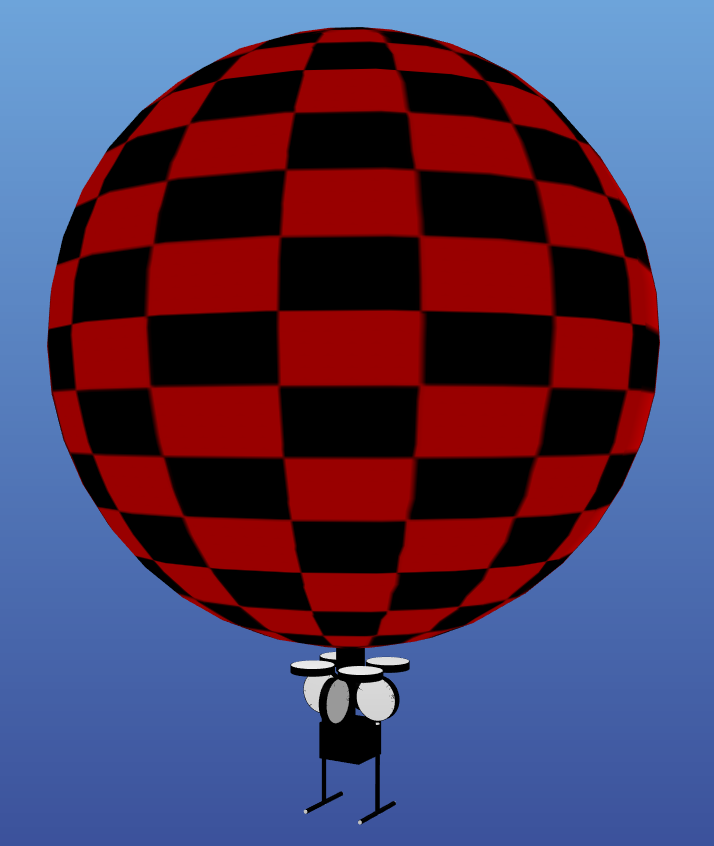
\includegraphics[width=0.5\textwidth]{blimp/blimp_crop.png}
    \caption{Simulated blimp. Model is about 3kg and has a
    balloon diameter of about 2m.}
    \label{fig:blimp_sim}
\end{figure}


\subsection{Hardware} \label{sec:quad_hardware}
Implementing these algorithms on actual hardware is obviously critical 
for this project. While a massive amount of work both in industry and 
academia has been done on the effective control of multicopters, most
existing autopilot or control stacks for multicopters consist of 
finely-tuned nested PID loops that take relatively high-level commands 
and then track them using low-level attitude, angular rate, and position 
controllers. To fully exploit the capabilities of the hardware platform, 
our method requires low-level control (i.e. independent motor commands) 
that is typically obscured in most control stacks. We therefore need to 
develop our own hardware platform with the compute power and communication
bandwidth required to solve the trajectory optimization problems and 
send low-level commands to the motors. This framework also naturally 
requires a good state estimate, so we plan on running these experiments 
in a motion-capture room and using a high-quality IMU 
(inertia measurement unit) and state estimator. 

Our goal is to release open-source designs for both the hardware and 
firmware required to run our emulator, so that others may easily benefit
from the versatility of the developed platform. 


\begin{figure}
    \centering
    \begin{subfigure}[b]{0.48\textwidth}
        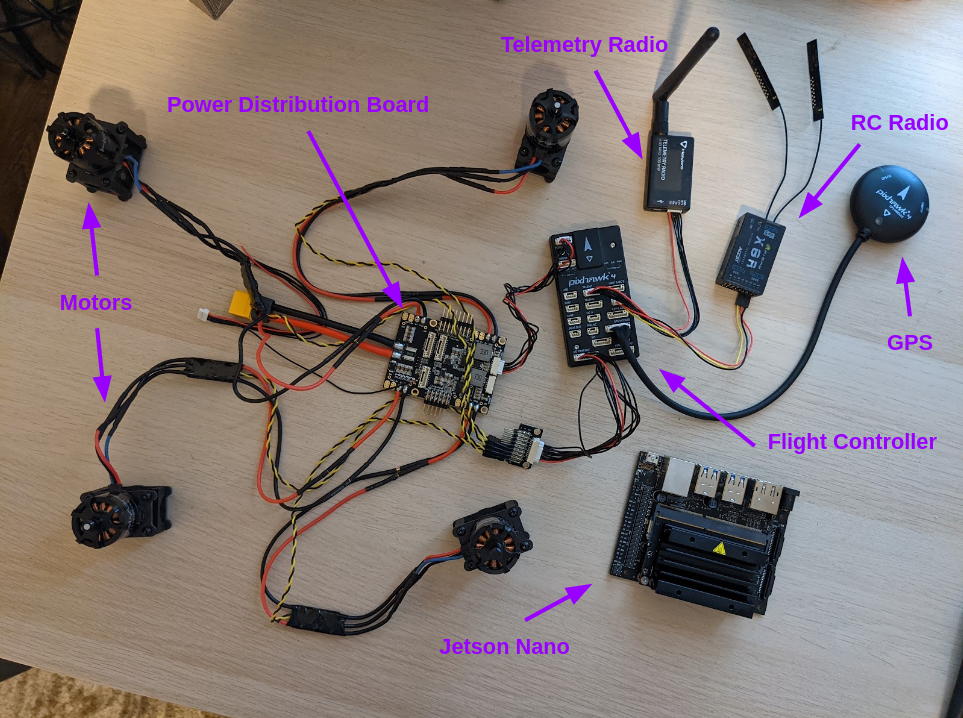
\includegraphics[width=\textwidth]{figures/blimp/quad_hardware_v1.png}
    \end{subfigure}
    \hfill
    \begin{subfigure}[b]{0.48\textwidth}
        \includegraphics[width=\textwidth]{figures/blimp/quad_x500.jpg}
    \end{subfigure}
    \caption{Preliminary hardware setup. Future revisions will likely 
    use a custom-printed PCB with built-in a built-in microcontroller
    and IMU, replacing the Pixhawk 4 shown here. An NVidia Jetson board
    will be used for the onboard compute module, which will communicate
    over serial to the microcontroller.}
\end{figure}

\begin{figure}
    \centering
    \begin{subfigure}[b]{0.48\textwidth}
        \includegraphics[width=\textwidth]{blimp/position_comp.tikz}
    \end{subfigure}
    \hfill
    \begin{subfigure}[b]{0.48\textwidth}
        \includegraphics[width=\textwidth]{blimp/attitude_comp.tikz}
    \end{subfigure}
    \caption{Trajectory comparison between the quadrotor (solid) and 
    blimp (dashed).}
    \label{fig:quadblimp_comp}
\end{figure}

\section{Preliminary Results} Using ALTRO (see Chap. \ref{chap:altro}), we
simulated a quadrotor emulating the dynamics for a small blimp (see Fig.
\ref{fig:blimp_sim}). We designed a simple LQR controller for the blimp that
stabilized it about the origin. Starting at rest from a position of $(1,1,1)$
and a yaw offset of $45^\circ$, the system had to move to the origin. The
position and attitude trajectories are compared in Fig.
\ref{fig:quadblimp_comp}. As shown these preliminary results look very good,
since the quadrotor, without any reference to the blimp trajectory shown,
achieves a very similar trajectory. Using a blimp sample rate of $0.5 s$, a
quadrotor sample rate of $10 ms$, and a total simulation time of $10 s$, the
problems solved in an average of 2.3 iterations and took an average of $2 ms$
on a laptop computer.

The preliminary algorithm is summarized in Algorithm \ref{alg:quad_emulator}.
The algorithm takes as inputs the discrete dynamics for the desired 
system $\hat{f}_d(\hat{x},\hat{u},T)$ with time step $T$, 
the discrete dynamics for the 
actual system (the quadrotor) $f_d(x,u,h)$ with time step $h$, and 
the control policy for the desired system $\Pi(\hat{x})$. On line 4, 
the controller runs the enclosed code every $T$ seconds.
On line 10, the control is extracted from the iLQR solver embedded in 
ALTRO, which stores a locally-optimal TVLQR (time-varying LQR) controller.
As a slight improvement on this algorithm, we've also implemented a version
that simulates the blimp some small number of steps into the future, and 
solves a longer trajectory optimization problem every $T$ seconds. Not 
only does this allow for some more strategic lookahead, it allows a time 
buffer since a valid tracking controller will still exist while the 
new trajectory is being calculated. 

\begin{algorithm}
\begin{algorithmic}[1] \label{alg:quad_emulator}
    \caption{Quadrotor Emulation}
    \State Given $f_d$, $\hat{f}_d$, $\Pi$, $h$, $T$
    \State $x \leftarrow$ initial quadrotor state
    \While{$t < t_sim$}
        \If{$\text{mod}(t, T) = 0$}
            \State $\hat{x} \leftarrow \textproc{Quad2Blimp}(x)$
            \State $\hat{x}' \leftarrow \hat{f}_d(\hat{x}, \Pi(\hat{x}),T)$
            \State Update problem with $\hat{x}$, $\hat{x}'$
            \State Solve problem
        \EndIf
        \State $u \leftarrow$ from iLQR tracking controller
        \State $x \leftarrow f_d(x,u,h)$, simulate quadrotor
    \EndWhile
\end{algorithmic}
\end{algorithm}

\section{Future Work}
There is a lot of work still to do on this problem. While the preliminary 
results are encouraging, there is still work to be done to get better 
dynamics matching. One possible avenue is to compute feedforward controls 
that attempt to match the desired accelerations expected by the dynamics.
Another, which was briefly mentioned previously, is to use an implicit 
integratator for the desired system and derive a low-order polynomial 
spline to use as a reference trajectory during the optimization solve,
instead of the more naive goal-based objective function used in the 
current implementation.

As mentioned in Sec. \ref{sec:quad_hardware}, a lot of work is still left to
be done to validate the algorithm on real hardware. The multicopter hardware
needs to be developed and tested, as well as developing a good control stack
for the blimp, which is currently housed at NASA JPL, who is sponsoring this
project. We also plan to apply this to other dynamical systems, such as the
Mars helicopter, to futher showcase its versatility.

Another interesting area of future work would be to use a fully-actuated
multicopter, since this would allow for better tracking performance, as well
as direct comparison against a simple feedback linearization scheme that
cancels the quadrotor dynamics and inserts the desired dynamics.

\end{document}